\vspace*{-0.2in}
\section{Results}

To validate our method, we use the Activities of Daily Living (ADL) dataset~\cite{Ramanan12}.  It is the largest available egocentric dataset for activity recognition, and to our knowledge, the most diverse and realistic.  It consists of hundreds of egocentric clips	(roughly 10 hours of video in total) collected from 20 people performing 18 actions in their own homes. These naturally
  occurring  actions are often related to hygiene or food preparation, e.g., combing hair, brushing teeth, doing laundry, washing dishes, etc. The authors also provide the object detector outputs from a part-based model~\cite{DPM} for 26 object classes, which we directly use as input to our method.  The objects include household items.  Five of the 26 detectors are for active versions of certain objects (namely, refrigerator, microwave, mug, oven/stove, and soap liquid).\footnote{The ADL dataset has been modified since the publication of
	\cite{Ramanan12}; because of this, running the published code gives
	slightly lower accuracy than the originally published numbers. We use the
  modified version of the dataset available from the authors webpage at the time of writing to
run all experiments.}  We use the authors' publicly available code to run their method for comparison.   
  
  
Throughout, we use five rounds of boosting and populate our candidate pool with 4-level pyramids.  Preliminary experiments showed that the finer-grained (4-level) pyramids were more often selected by boosting than their coarser 3-level counterparts, so we focus the pool accordingly for all results.  

  %
%  The work of \cite{Jiang12}, which uses a similar
%  pyramid-based boosting approach for 2D image recognition, found that using
%  pyramids with more than 3 levels actually led to a decrease in overall
%  accuracy due to over-segmentation of image space. However, we found that in the
%  3D case 4-level pyramids give better overall accuracy than coarser-grained
%  representations.

%  Object detectors are trained on videos from the
%  first 6 people and tested on the videos from the remaining 14 people.
%
%\begin{table}
%  \begin{center}
%\begin{tabular}{cc}
%\bmvaHangBox{\fbox{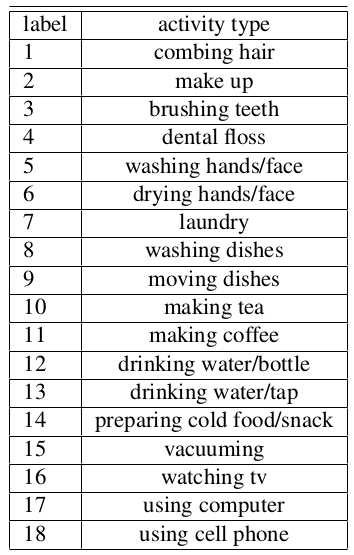
\includegraphics[width=4.0cm]{figures/actionlist.png}}}&
%\bmvaHangBox{\fbox{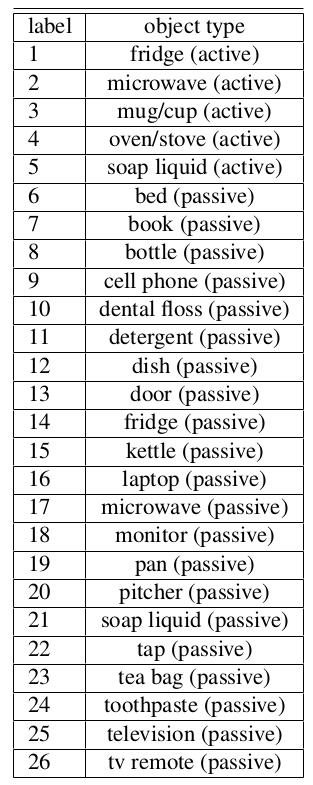
\includegraphics[width=4.0cm]{figures/objectlist.png}}}\\
%\end{tabular}
%		   \caption{Lists of action types and object types present in the
%       ADL dataset. Separate active and passive models are trained for fridge,
%     microwave, mug/cup, oven/stove, and soap liquid.}
%\label{fig:teaser}
%  \end{center}
% \end{table}


%
%	Each frame in the dataset
%	is annotated with activity labels and bounding boxes for detected objects and hand positions,
%	Additionally, each object is tagged as active or passive depending
%	on whether it is being interacted with.
%
%  One difficulty that can arise within egocentric
%  activity recognition is that activities can be temporarily interrupted by
%  other activities. For instance, while waiting for tea to brew a subject
%  may watch TV. For cases of such interruptions, to avoid unnecessary
%  complications resulting from frames being annotated with multiple
%  activities, the ADL dataset simply uses the label of the interrupting
%  action when a longer action is disrupted.


  We follow the exact evaluation protocol given in~\cite{Ramanan12}.  Specifically, we evaluate recognition accuracy using leave-one-person out: we test on videos from each person $i$ in turn, having trained on all remaining people.  We exclude the first 6 people, since their data was used to train the object detectors.
  
  
Table~\ref{table:results} shows the results, in terms of the average recognition rate over all 18 action classes.  We compare our boosted RSTP+OCC approach to four baselines.  The first baseline, bag-of-words (BoW), uses space-time interest points and HoG/HoF visual words, and represents what is now a standard representation for third-person action recognition.  The second baseline uses a bag-of-objects.  The third baseline, the Temporal Pyramid, is the method proposed in~\cite{Ramanan12}, and represents the state of the art on this dataset.  The fourth baseline, RSTP, is just like the proposed approach only it lacks the object-centric cuts.

Our approach outperforms all four baselines and improves the state of the art.  Compared to BoW, we have the advantage of high-level object-based features.  While the Temporal Pyramid~\cite{Ramanan12} also has this benefit, it is weaker than our method due to its reliance on a hand-crafted pyramid structure.  Notably, the proposed object-centric cuts are essential for our strong recognition result.  Simply using  boosting with purely randomized partitions (RSTP) is noticeably weaker.  This supports our claim that it is useful to bias bins according to object interactions for egocentric data.


  \begin{table}
		\begin{center}
			\begin{tabular}{|l|c|c|c|c|c|}
				\hline
        BoW & Bag-of-objects & TempPyr~\cite{Ramanan12} & Boost-RSTP & Boost-RSTP+OCC (ours) \\
				\hline\hline
        16.5\% & 34.9\% & 36.9\% & 33.7\% & \textbf{38.7\%}\\
				\hline
			\end{tabular}
		\end{center}
		\caption{Overall classification accuracy on ADL. Our method improves the state of the art.}\label{table:results}
	\end{table}

%
%
%  \begin{figure}
%  \begin{center}
%  \bmvaHangBox{\fbox{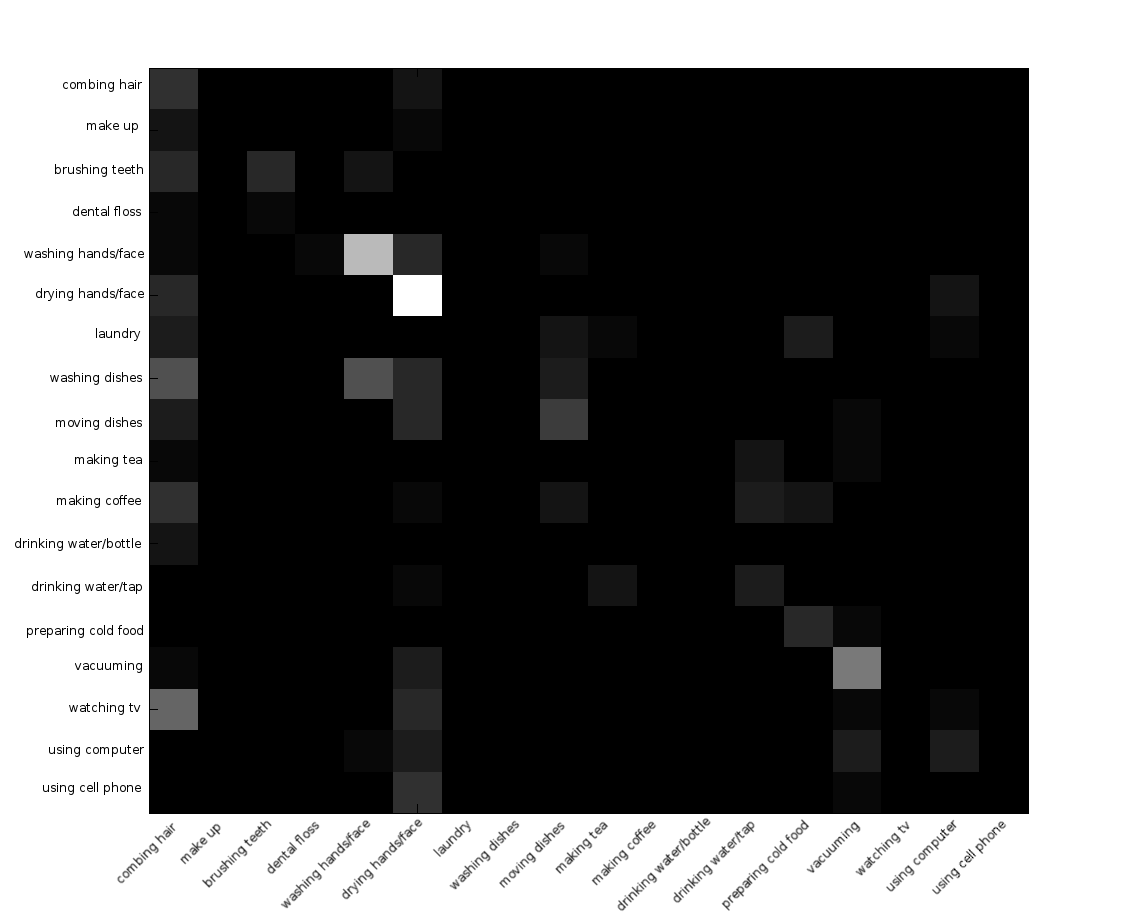
\includegraphics[width=6.0cm]{figures/confn2-labels.png}}}
%		   \caption{Confusion matrix for RSTP+OCC using detected active and
%       passive objects}
%  \label{fig:teaser}
%  \end{center}
%  \end{figure}



Looking more closely at our method's predictions, we find it has particularly good accuracy for ``combing hair'' and ``drying  hands/face''.  This suggests that the learned bins were able to usefully isolate the regular space-time relationships these actions exhibit.  On the other hand, we often confuse ``making tea'' and ``making coffee'', likely because they involve the same active objects.   Furthermore, since the distributions of objects across space-time are similar for both, and kettles and tea bags are not modelled as active objects, it is
  difficult for our boosting algorithm to select partitions that
  are discriminative for these classes. An extension of our method which
  allows selecting partitions on a per-class basis
  could allow for more fine-grained control and could help mitigate such
  issues, though would be more expensive.  We leave this as future work.


Compared to the Temporal Pyramid~\cite{Ramanan12}, we find out method is especially stronger for ``combing hair", ``brush teeth", ``dental floss".  This indicates that our learned spatial cuts are essential in scenes with similar objects appearing across different actions, as is the case with these bathroom-based activities.  For instance, while combing hair, floss or toothpaste might appear on the
counter, but floss or toothpaste would appear higher in the field of view when actually in use.







\begin{figure}
  \begin{center}
  \begin{tabular}{cc}
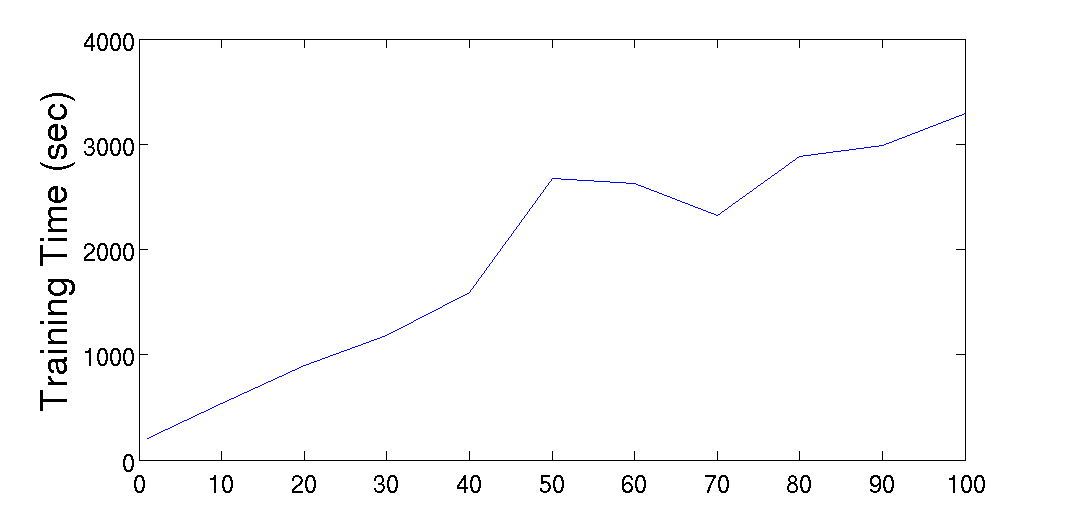
\includegraphics[width=5.2cm]{figures/runtime.png}
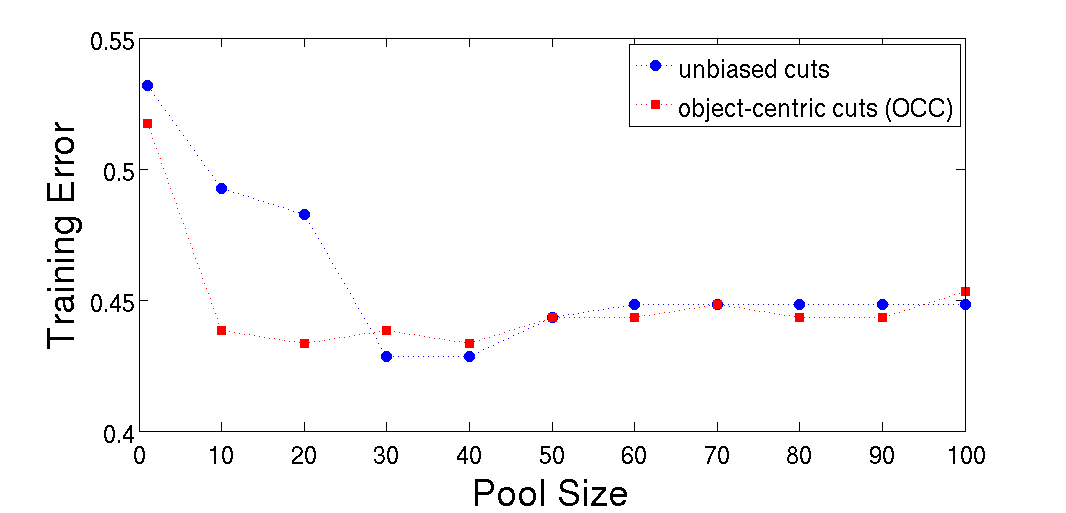
\includegraphics[width=5.2cm]{figures/trainerror.png}
\end{tabular}
		   \caption{Left: Training time as a function of pool size.  Right: Training error as function of pool size, for both uniformly sampled random shifts and the proposed object-centric partitions.  By focusing on object-centric shifts, we can achieve a stronger classifier with a smaller total pool, which improves training efficiency.}\vspace*{-0.1in}\label{fig:runtime-trainerror}
  \end{center}
\end{figure}

Figure~\ref{fig:runtime-trainerror} emphasizes the benefits of object-centric cuts.  On the left, we show the training time of running boosting with increasingly larger pools of candidate pyramids, averaged over five runs; run-time increases linearly with pool size.
On the right, we show the training error as a function of the pool size.  As desired, we see that the object-centric cuts lead to lower error with smaller pool sizes, compared to the unbiased RSTP's.  Essentially, our method focuses the pool on those candidates that \emph{a priori} have good chance at capturing discriminative aspects of the object distribution in space-time.  Thus, fewer total candidates must be explored to find good ones, and we can train the models with less total training time.

%  Larger improvements are visible with smaller pool sizes, and the difference
%  between the two pools diminishes as pool size increases. This conforms to
%  expectations because as the unbiased pool grows in size, it becomes more
%  likely to contain discriminative partition schemes, while the biased pool
%  is forced to contain discriminative partition schemes even at relatively
%  small pool sizes. This result suggests that by using object-centric
%  partitions rather than unbiased partitions, we can obtain good recognition
%  results even with a smaller pool, making our boosting algorithm less expensive
%  to compute.
%
%  \begin{figure}[t]
%		\begin{center}
%			%\fbox{\rule{0pt}{2in} \rule{0.9\linewidth}{0pt}}
%			  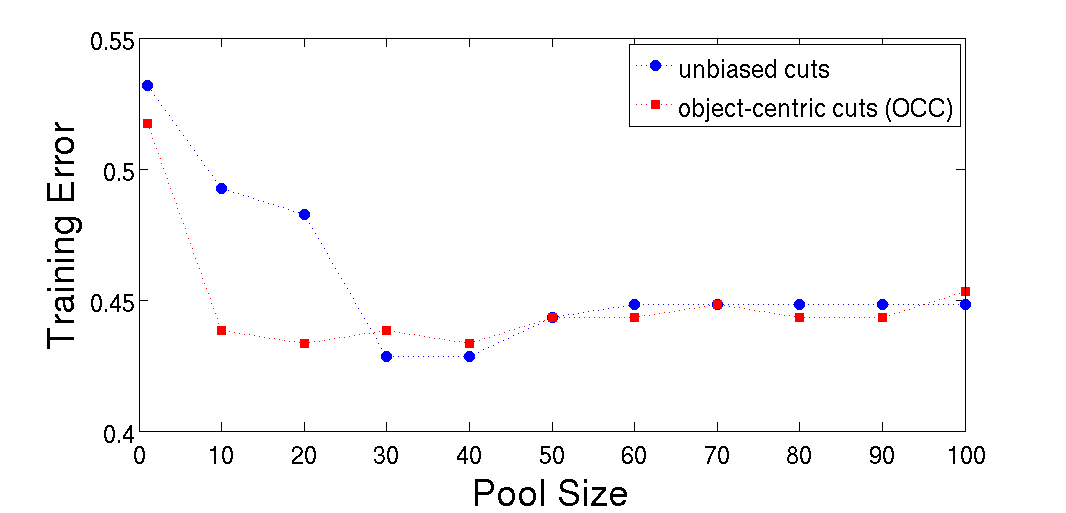
\includegraphics[width=1.0\linewidth]{figures/trainerror.png}
%		\end{center}
%		   \caption{Effect of using biased partition schemes. The object-centric
%         pool
%       usually has lower training error
%       than the pool of unbiased partition schemes. The most significant
%     improvement is visible at smaller pool sizes.}
%				\label{fig:long}
%				\label{fig:onecol}
%	\end{figure}
%
%	